\documentclass[12pt]{article}
\renewcommand{\baselinestretch}{1.4}
\usepackage{amsthm,amssymb,amsmath,graphicx}
\usepackage{color}
\usepackage{url}
\usepackage[top=2cm, bottom=2cm, left=2cm, right=2cm]{geometry}
\usepackage[pagebackref=false,colorlinks,linkcolor=blue,citecolor=blue]{hyperref}
\usepackage{babel}
\usepackage{blindtext}
\usepackage{graphicx}
\usepackage{subcaption}
\setlength{\parindent}{0pt}
\usepackage[localise=on]{xepersian}
\usepackage{xepersian}
\settextfont{IRMitra}

\makeatletter
\newcommand{\xRightarrow}[2][]{\ext@arrow 0359\Rightarrowfill@{#1}{#2}}
\makeatother

\newcounter{mynumber}
\setcounter{mynumber}{1}
\newcommand{\mynum}{\arabic{mynumber}\stepcounter{mynumber}}
\newenvironment{ques}[0]{\textbf{سوال \mynum.}}{}
\newtheorem{قضیه}{قضیه}

\title{حل تمرین فصل اول، بخش دوم}
\author{
	ساختمان داده ها و الگوریتم
	\\
	سجاد هاشمیان 
}
\date{زمستان ۱۳۹۹}

\begin{document}
	\maketitle
	\setRTL 

	\begin{ques}
		\\
		با کمک از سری هارمونیک داریم:
		$$
		T(n)=\sum_{i=1}^{n} i+\frac{1}{i}=\sum_{i=1}^{n} i+\sum_{i=1}^{n} \frac{1}{i}=
		\frac{n(n+1)}{2}+\mathcal{H}_n=\Theta(n^2)+\Theta(\ln n)=\Theta(n^2+\ln n)=\Theta(n^2)
		$$
	\end{ques}
	\begin{ques}
		\\
		\textbf{يادآوری(قضیه اصلی، حالت دوم).}
		$
		T(n)=aT(\frac{n}{b})+f(n):
		f(n) = \Theta(n^{\log_b a}) \Longrightarrow T(n) = \Theta(n^{\log_b a}\log n)
		$
		\\
		با توجه به تعریف سوال از $T(n)$
		داریم: $a=2,b=4,f(n)=\sqrt{n}=n^\frac{1}{2}$
		، بنابراین این تابع در شرایط قسمت دوم قضیه اصلی صدق می‌کند و طبق آن 
		$T(n)\in\Theta(\sqrt{n}\log n)$
		است.
	\end{ques}
	\begin{ques}
		$
		T(n) = T(\frac{n}{2}) + T(\frac{n}{3}) + T(\frac{n}{4}) + n^2
		$
		\begin{flushleft}
		$
		\begin{cases}
		T(n)<3T(\frac{n}{2})+n^2 \xRightarrow{\log_2 3<n^2} T(n)\leq \Theta(n^2)\Rightarrow T(n)\in O(n^2)
		\\
		T(n)>3T(\frac{n}{4})+n^2 \xRightarrow{\log_4 3<n^2} T(n)\geq \Theta(n^2)\Rightarrow T(n)\in \Omega(n^2)
		\end{cases}	\Longrightarrow T(n)\in \Theta(n^2)
		$
		\end{flushleft}
		
	\end{ques}

	\begin{ques}
		\\
		ابتدا رابطه بازگشتی را با تغییر متغییر 
		$k=\sqrt{m}$
		به شکل زیر بازنویسی می‌کنیم:
		$$T(n)=\begin{cases}
			8T(\frac{n}{2})+\Theta(1)&n>k\\
			k^2& n<k
		\end{cases}$$
		حال با استفاده از مجموع در درخت بازگشت رابطه فوق داریم:
		$$
		T(n)\in\Theta\Bigg(\sum_{i=0}^{\log \frac{n}{k}} 8^i \frac{n}{2^i}\Bigg)
		=\Theta\Bigg(n\sum_{i=0}^{\log \frac{n}{k}} 4^i\Bigg)
		$$
		اما باید $g(n,k)=\sum_{i=0}^{\log \frac{n}{k}} 2^{2i}$
		را محاسبه کنیم:
		\\
\newpage
		\textbf{محدود کردن حاصل جمع‌ها با انتگرال}\quad$\sum_{i=1}^n f(i)\leq \int_1^{n+1} f(x)dx$
		\\
		با توجه به رابطه فوق 
		$g(n,k)=\Theta(\int 2^{2i})$
		که با حل انتگرال فوق داریم:
		$$
		g(n,k)=\Theta(2^{\log\frac{n^2}{k}})\in \Theta(\frac{n^2}{k})$$
		\\
		\textbf{محاسبات پایه لگاریتم ها}\quad$\log(a+b)=\log(a(1+\frac{b}{a}))=\log a+\log(1+\frac{b}{a})$
		\\
		طبق رابطه گفته شده، داریم:
		$$\log(g(n,k))=\log(2^{2\log 2})+\log(g(n-k,k))$$
		$$(\log o\:g)(n,k)=(\log o\:g)(n-k,k)+4$$
		از آنجا که
		$k$
		به عنوان پارامتر ثابت تکرار می‌شود، قابل حذف است؛
		بنابراین طبق قضیه اصلی و سپس حذف تابع لگاریتمی که در ابتدا محاسبات اضافه کردیم
		داریم:
		$g(n)\in \Theta(\frac{n^2}{k})$
		\\
		درنهایت
		با توجه به محاسبات فوق داریم:
		$T(n)\in \Theta(n)\times \Theta(g(n))=\Theta(\frac{n^3}{\sqrt{m}})$
	\end{ques}
\\
	\begin{ques}
		\begin{flushleft}
			$
			U(m)=T(2^m)=T(\frac{2^m}{2})+\log (2^m)=T(2^{m-1})+m=U(m-1)+m
			$
		\end{flushleft}

	\end{ques}

	\begin{ques}
		\\
		کافیست تا اعداد را در بلوک های $\sqrt{n}$
		تایی به ماشین ورودی دهیم، در اینصورت 
		$\sqrt{n}$تا
		بلوک به اندازه $\sqrt{n}$
		داریم؛ که هر کدام از آنها طبق فرض سوال از مرتبه
		$O(1)$
		قابل محاسبه و همینطور 
		از $O(1)$
		قابل ترکیب با دیگر بلوک ها است،
		و این یعنی از مرتبه 
		$\sqrt{n}$
		می‌توانیم این دو عدد را در هم ضرب کنیم که کمترین گزینه موجود است.
		\begin{figure}[h!]
			\centering
			\begin{subfigure}[b]{\linewidth}
				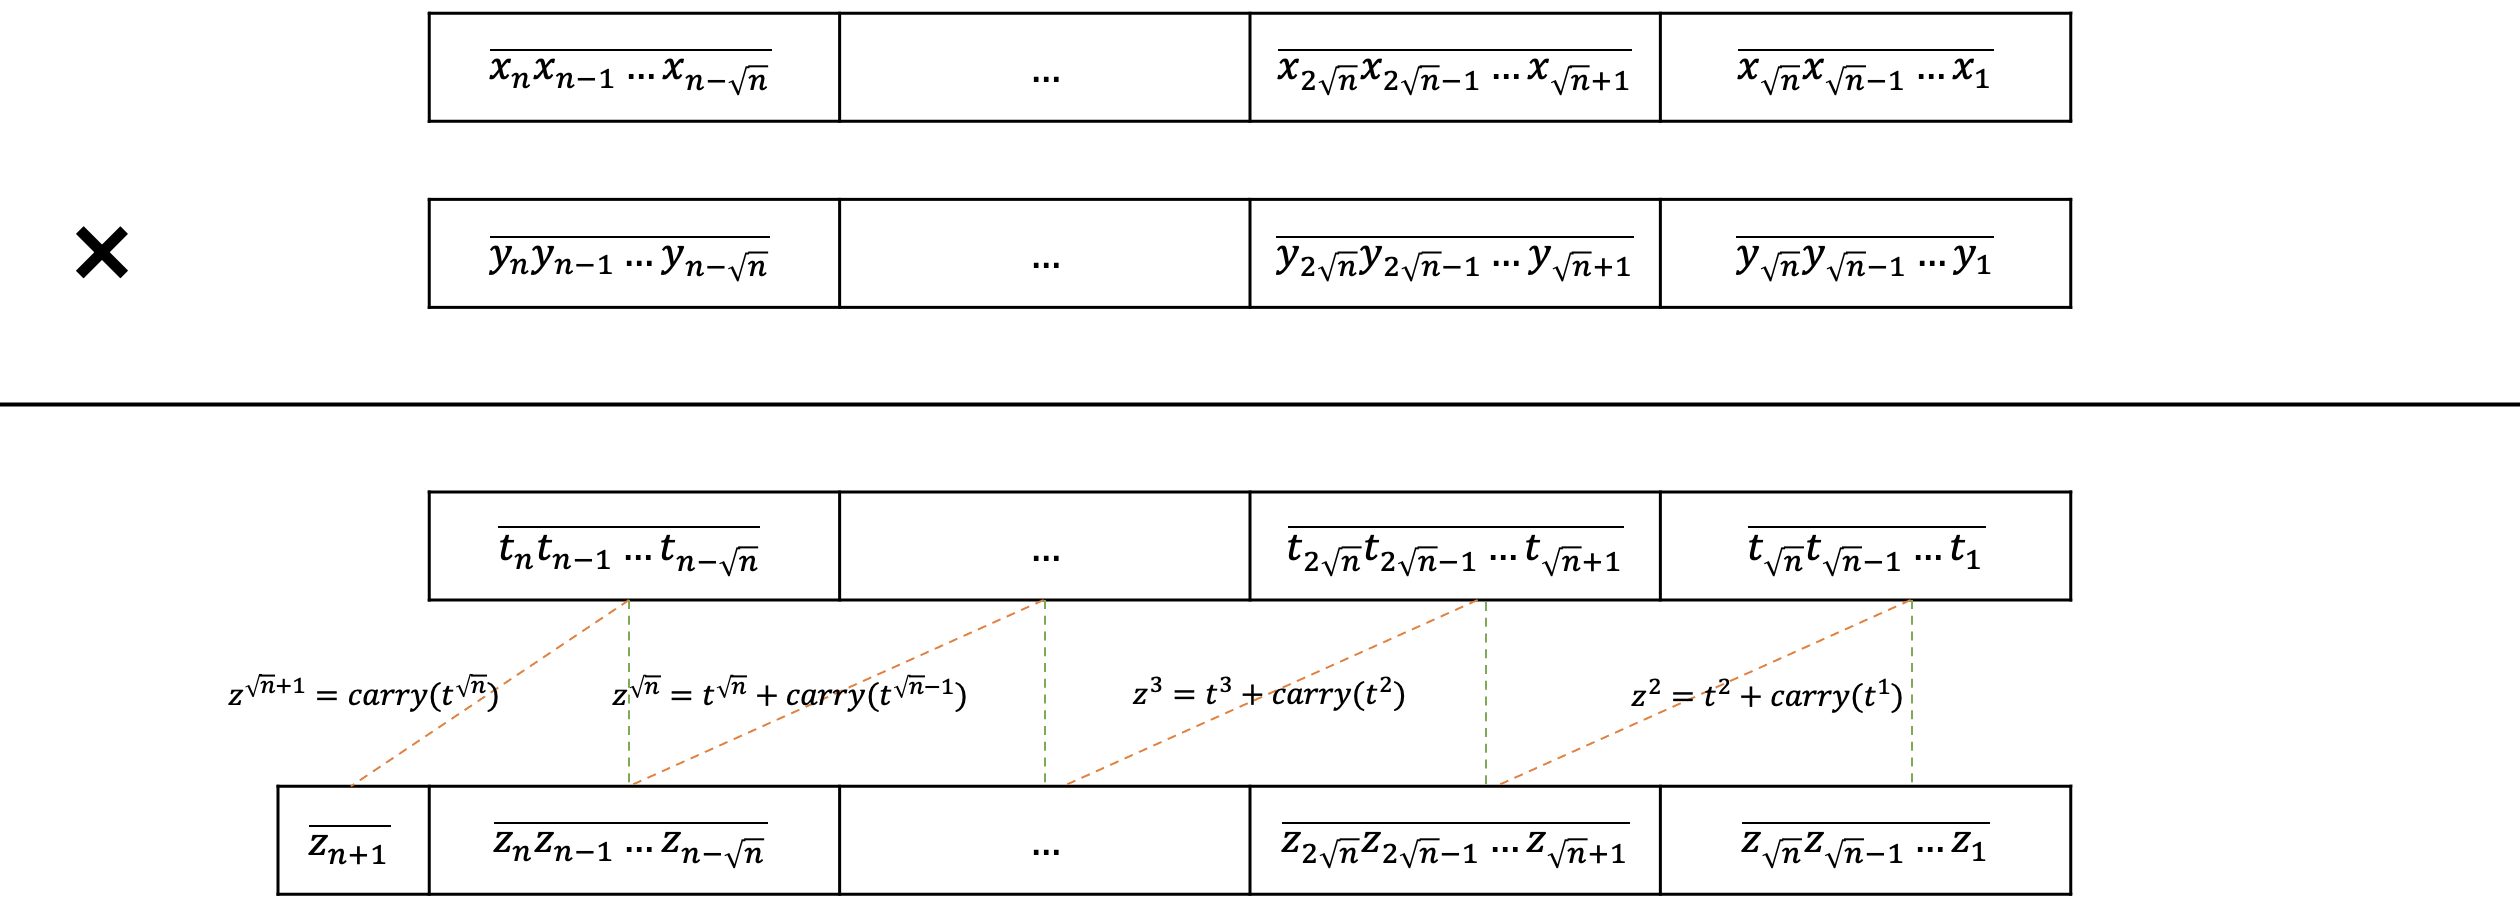
\includegraphics[width=\linewidth]{img2.png}
			\end{subfigure}
			\end{figure}
		\end{ques}

	\begin{ques}
		\\
		آیا رابطه ای بین این تابع بازگشتی و مسئله زیر می‌بینید؟
		\\
		\textbf{مسئله:}
		با استفاده از یک نخ به طول 
		$2\alpha+2\beta$
		یک چهار‌ضلعی ساخته‌ایم، مساحت بیشینه چهار‌ضلعی
		ممکن چقدر است؟

	\end{ques}


\end{document}